\chapter{Descriptions of the Southern Sample}
	\label{cha:Description}
In this appendix we describe our observations as well as those of the literature for each galaxy in our Southern sample. Unless otherwise stated, all galaxies have stellar populations which are old, metal-rich and alpha-element enhanced.

\textbf{ESO 443-G24} has a co-rotating, kinematically-decoupled core (KDC). Both the core and the outer parts of the galaxy rotate with very low velocities ($\approx 20\,\mathrm{km\,s^{-1}}$). The [\ion{O}{iii}] emission line doublet is only detected at the centre of the galaxy, while H\,$\beta$ is only detected when the whole field of view is integrated. 

\textbf{IC 1459} is known to contain a KDC \citep{Franx1988} embedded in a slow rotator. This is clearly seen in both the VIMOS and MUSE mean velocity maps (Figs. \ref{fig:VIMOS_stellar} and \ref{fig:MUSE_stellar}). It is also known to have ionized gas counter rotating with respect to the decoupled core \citep{VerdoesKleijn2000}. This is again seen by comparing Fig. \ref{fig:VIMOS_stellar} with \ref{fig:VIMOS_Gaskine} and \ref{fig:MUSE_stellar} with \ref{fig:MUSE_Gaskine}. \citet{Franx1988} claim that the gas is rotating in the same direction as the outer part of the galaxy, though this is not clear from our mean velocity maps. We speculate that the gas is likely to be of external origin, although we propose a mechanism whereby it may have been stripped from the progenitor galaxy in the merger which resulted in the KDC, before being re-accreted and thus has an internal origin. The ionizing radiation field originates from the AGN and gives a low-ionization nuclear emission-line region (LINER) classification.

Figure \ref{fig:ic1459radio} shows that the radio spectral energy distribution (SED) for IC 1459 has a gigahertz peak spectra (GPS). These are general taken to be indicative of a recently turned on radio jet residing in a gas-rich environment \citep[e.g.][]{ODea1998}. 

\begin{figure}
	\centering
	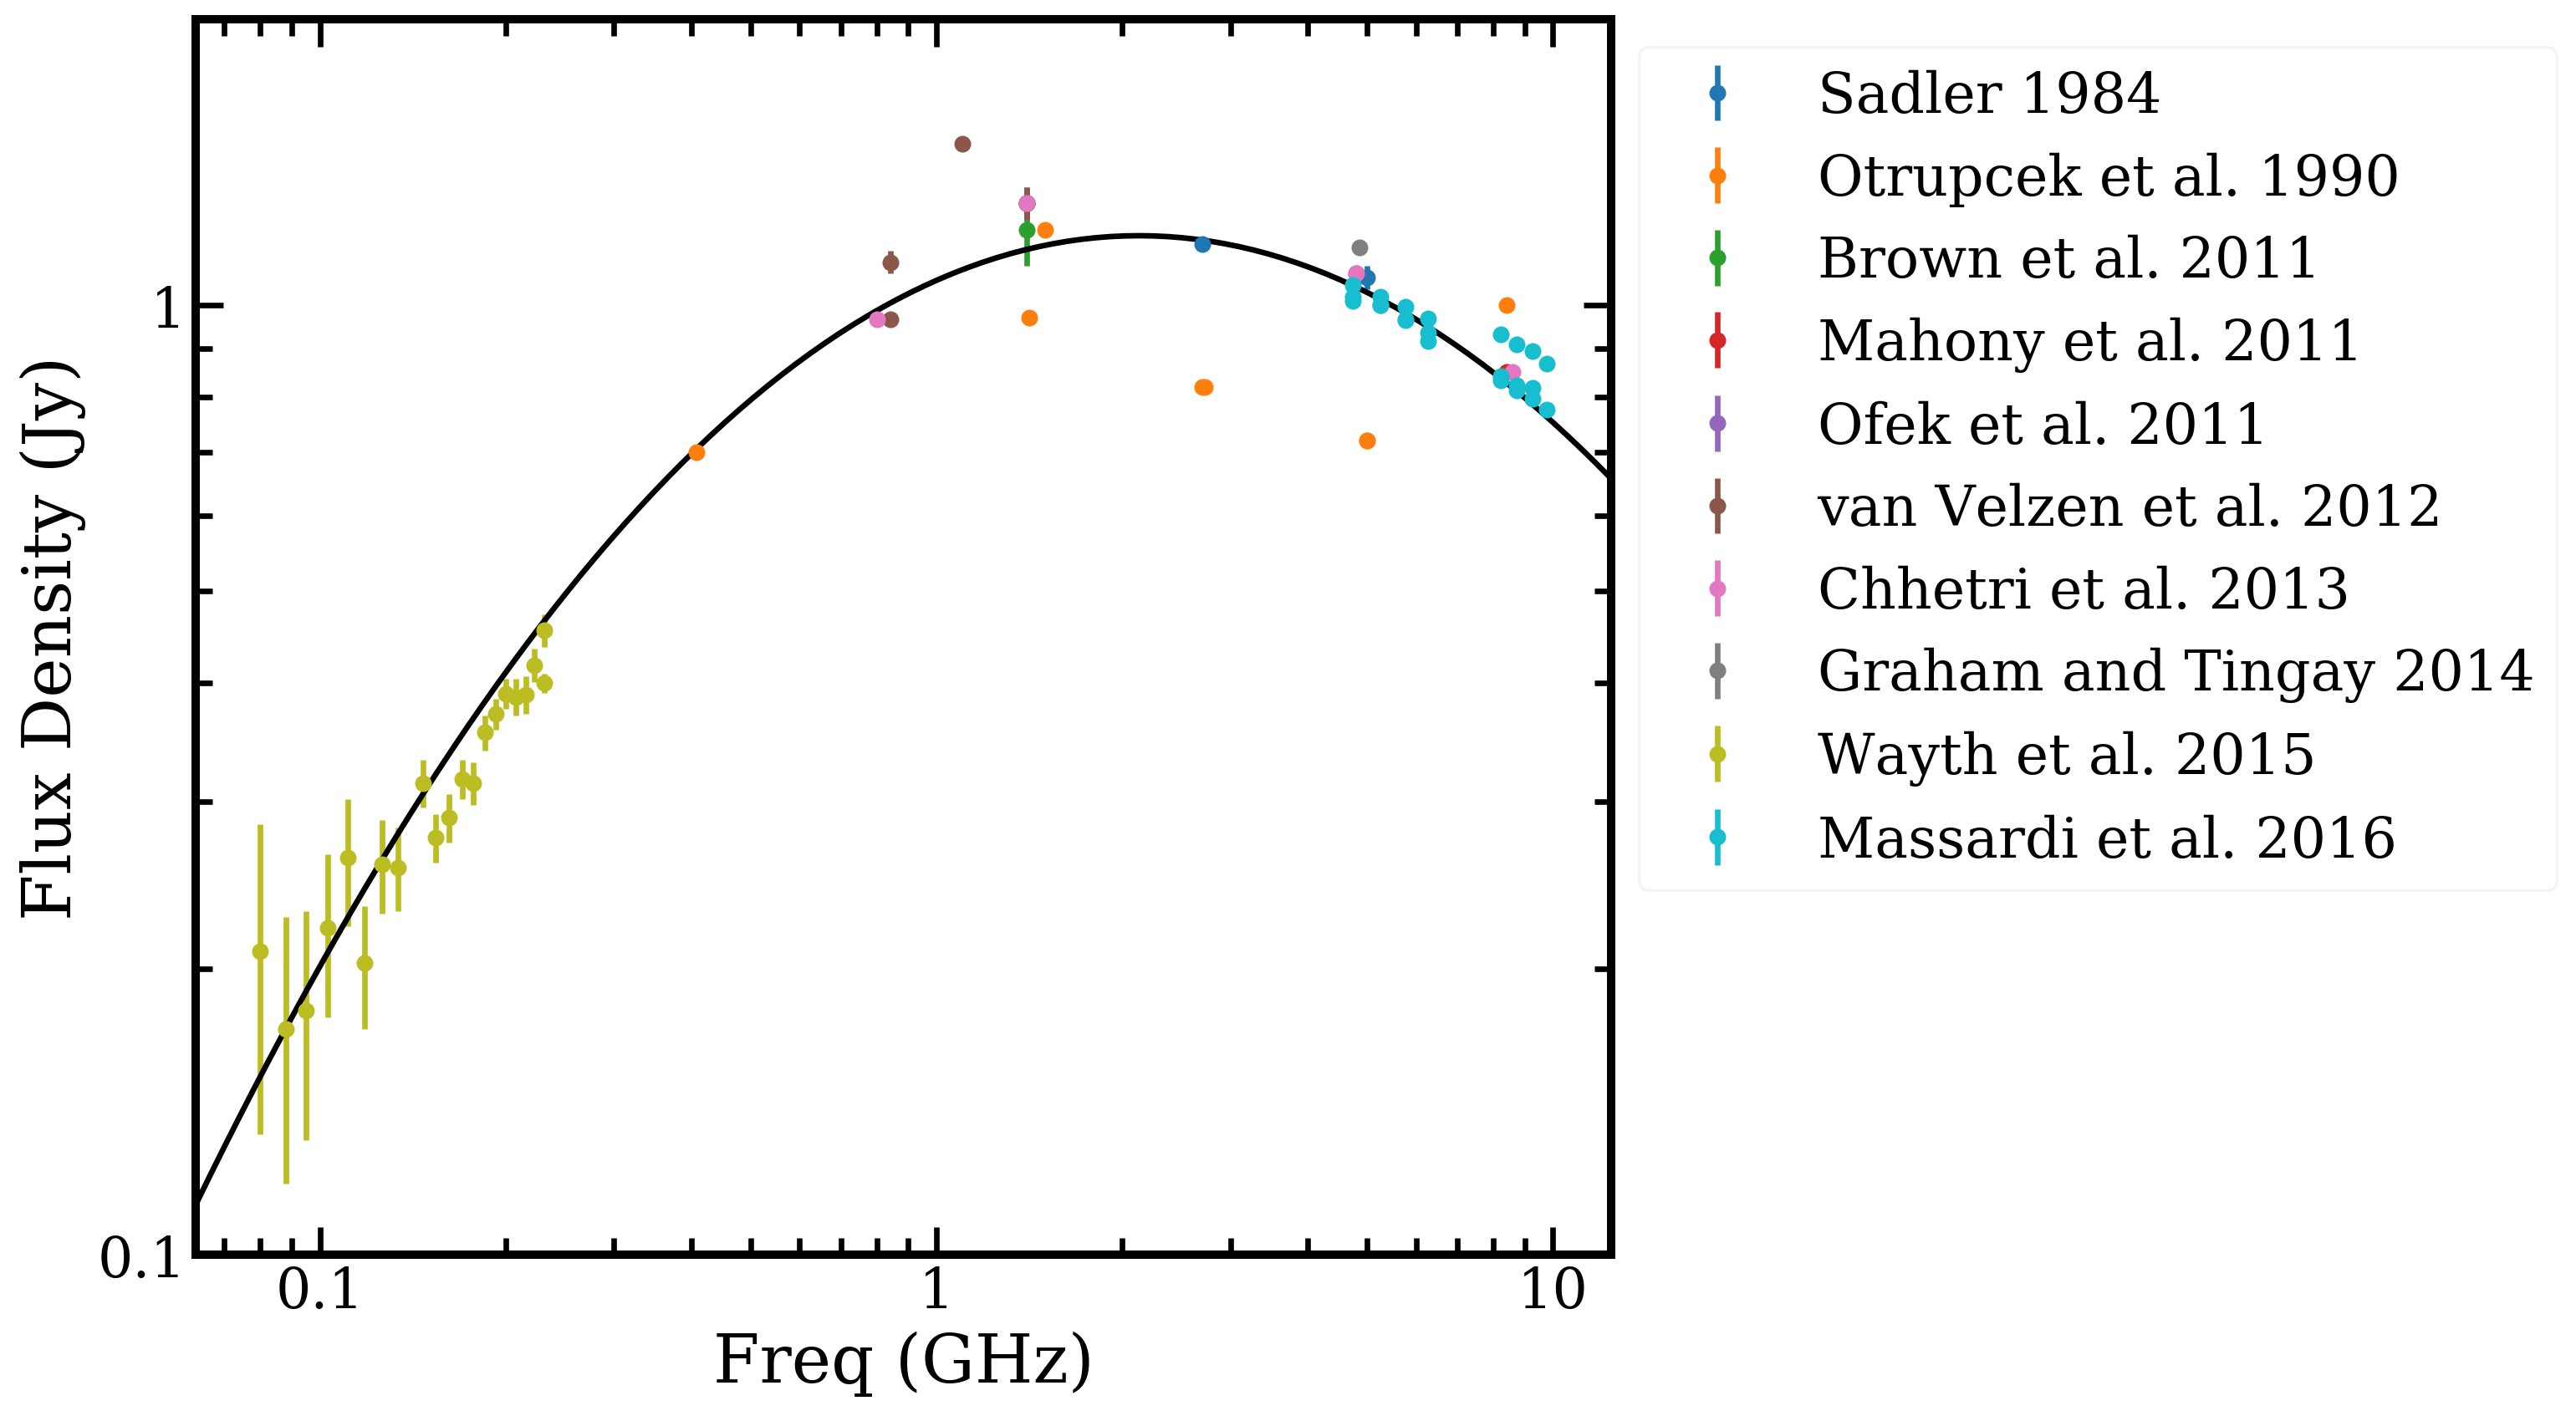
\includegraphics[height=0.4\textwidth]{appendix/appendix2/ic1459.png}
	\caption[Radio SED for IC 1459]{Radio SED for IC 1459 showing it to be a GPS source. Different colour indicate different papers as indicated in the legend. The black line is to guide the eye. Data collected using the VizieR database via the CDS portal tool \citep{Ochsenbein2000}.} 
	\label{fig:ic1459radio}
\end{figure}
\nocite{Brown2011, Massardi2016, Ofek2011, Wayth2015, Mahony2011, Otrupcek1990, Graham2014, Chhetri2013, VanVelzen2012, Sadler1984}

\textbf{IC 1531} is a slow rotator with very low mean velocities. The ionized gas is only detected in the central regions and is classified as one of two Seyfert 2 galaxies in our Southern sample, although it has quite weak H\,$\beta$ equivalent widths. 

\textbf{IC 4296} is a slow, but regular rotator. Its ionized gas is only detected in the centre of the galaxy with LINER characteristics. The source of the ionizing radiation field is attributed to the AGN. 

\textbf{NGC 612} has a large dust lane to the east of the apparent center of the galaxy and perpendicular to the axis of rotation. It has very high rotational velocities for a massive ETG, with an extended CO disc and a younger stellar population. All this suggests that NGC 612 may have a very different history to the rest of the Southern Sample. We have shown (in agreement with others e.g. \citealt{Ledlow1998} and \citealt{Emonts2009}) that it is one of only a handful of known disc-dominated radio (AGN) galaxies \citep[e.g.][]{Morganti2011}. Spiral hosts are even rarer with only 4 known cases \citep{Ledlow1998, Hota2011a, Bagchi2014, Mao2015}, although they might much more difficult to detect against the background radio emission from star formation within the spiral.

With the dust lane obscuring much of the galaxy (including its very centre) it is difficult to observed trends within the galaxy. However, the absorption line maps (other than H\,$\beta$) appear to be misaligned with the surface brightness (see Fig.\,\ref{fig:VIMOS_absorption}). The peak of the absorption line strength maps, usually at the centre of the galaxy, is instead found to the west of the peak surface brightness with the presumed centre of the galaxy to the east. Further study at higher spatial resolutions may resolve significant substructure to this galaxy. For the time being, it is clear that this galaxy is in a class of its own within our Southern sample. 

\textbf{NGC 1316} (Fornax A) was not observed with VIMOS, however the MUSE maps show it to be disturbed, but clearly rotating. At $\approx 2$\,Gyr, it has the youngest stellar population in our Southern sample. The ionized gas is spatially extended, but the kinematics are very messy and difficult to interpret. We suggest that the gas has similar kinematics to the stars, overlaid with a high velocity inflow almost perpendicular to the radio jet. We do however, concede that it is not clear and that other interpretations are possible. 

\citet{Lanz2010} observe spatially-coincident radio lobes and cavities in the X-ray gas., They interpret that the different spatial sizes of the radio lobe and X-ray cavity to mean that they are from separate outbursts 0.4 and 0.1 Gyr ago, respectively.

\textbf{NGC 1399}, the central galaxy of the Fornax Cluster \citep{Jordan2007}, is known to have kinematic twist (see MUSE map by Vaughan 2018 in prep.) on the scale of our MUSE field of view (reduced to 30"). We detect very little ionized gas, but that which we do detect has LINER characteristics. 

As in NGC 1316 by \citet{Lanz2010}, \citet{Su2017} observes spatially-coincident radio lobes and X-ray cavities. They also observe a potential third cavity (or bubble) thought to have previously inflated and become detached from the galaxy. This is known as a `ghost' bubble and shows evidence of past activity.

\textbf{NGC 3100} is a normal fast rotator with rotation about the semi-minor axis of the photometry i.e. the position angle of the stellar kinematics and photometry are aligned. However, both the ionized and the molecular gas is rotating about the semi-major axis. The molecular gas appears to form a broken ring about the centre of the galaxy with gaps spatially coincident with the radio lobes (Ruffa 2018 in prep.). The two peaks in the surface brightness of the ionized gas are also spatially coincident with the radio lobes. The ionized gas properties of NGC 3100 mean that it is one of the two galaxies in this sample classified as a Seyfert 2. 

\textbf{NGC 3557} is another massive fast rotator. It has very little ionized gas, which is concentrated 1--2$^{\prime\prime}$ away from the peak of stellar surface brightness. NGC 3557 is classified as a LINER galaxy, but the weakness of the H\,$\beta$ equivalent width means this cannot be attributed to the AGN. The stellar population shows a confined young ($\approx 5$\,Gyr) core. Since this galaxy has a relatively high stellar velocity dispersion, it is not clear how this core is maintained. 

\textbf{NGC 7075} is a slow rotator with a little centrally-concentrated, ionized gas. The emission-line properties have LINER characteristics, but we are unable to say if this is due to the AGN.

\textbf{PKS 718-34} possibly contains a KDC. Its distance means that we do not have a high enough signal-to-noise ratio (S/N) in the outer parts of the field of view for a conclusive classification. If true, PKS 718-34 would fit the KDC age--size relation found by \citet{Kuntschner2010}, although it would be one of the largest KDCs observed. The velocity dispersion map could also be interpreted as double peaked (2$\sigma$) indicative of counter-rotating discs. Such galaxies can also appear like a KDC \citep[e.g.][]{Bois2011}.
